\section{Introduction}
As this thesis is primarily an exploration of epitaxial interfaces using a wide array of experimental techniques, the background material here will cover the theoretical concepts that are regularly drawn upon to present the growth models presented elsewhere. Models presented later in the document are primarily of a conceptual nature and as such background here will also be presented in that manner. Mathematics will be used where applicable but will be generally avoided, as the restricted assumptions are of little use to the work presented later.

There are a few key theoretical concepts which must be understood in order to best describe the expanded epitaxial model proposed here. The first, and most integral to the discussion is an examination of the model of epitaxy as currently defined in the literature. This is integral to differentiate where the material systems examined diverge from the idealized models presented in the literature. As part of the examination of epitaxy, particular attention will be given to nucleation and clusters on surfaces as this examination hinges on the role of the epitaxial interface. Beyond epitaxy, the other key subjects which require background exposition are surface reconstructions, which describe the properties of the other side of the epitaxial interface, the substrate, and atomic bonding, the connections which reach across the epitaxial interface.

\section{Epitaxy}
\subsection{Homoepitaxy}
Equilibrium versus kinetics. Even the most perfectly matched systems in terms of atomic bonding and lattice match can grow with defects if the deposition rate is too fast.

\subsection{Heteroepitaxy}
%SiGe as the model system.
%
%Alignment using [HKL]//(hkl);[UVW]//[uvw] = film-up/substrate-up;film in-plane//substrate in-plane
%
%Sub and superlattice alignment
\begin{figure}
    \centering
    \missingfigure{Figure from ohring page 426 - Heteroepitaxy alignment}
    \caption{\label{fig:back_hetero_alignment}Simple epitaxial alignment of cubes on cubes\cite{Palmstrom1995}}
\end{figure}
%III-V lattice matched as next best model system
\subsubsection{Strain}
\begin{figure}
    \centering
    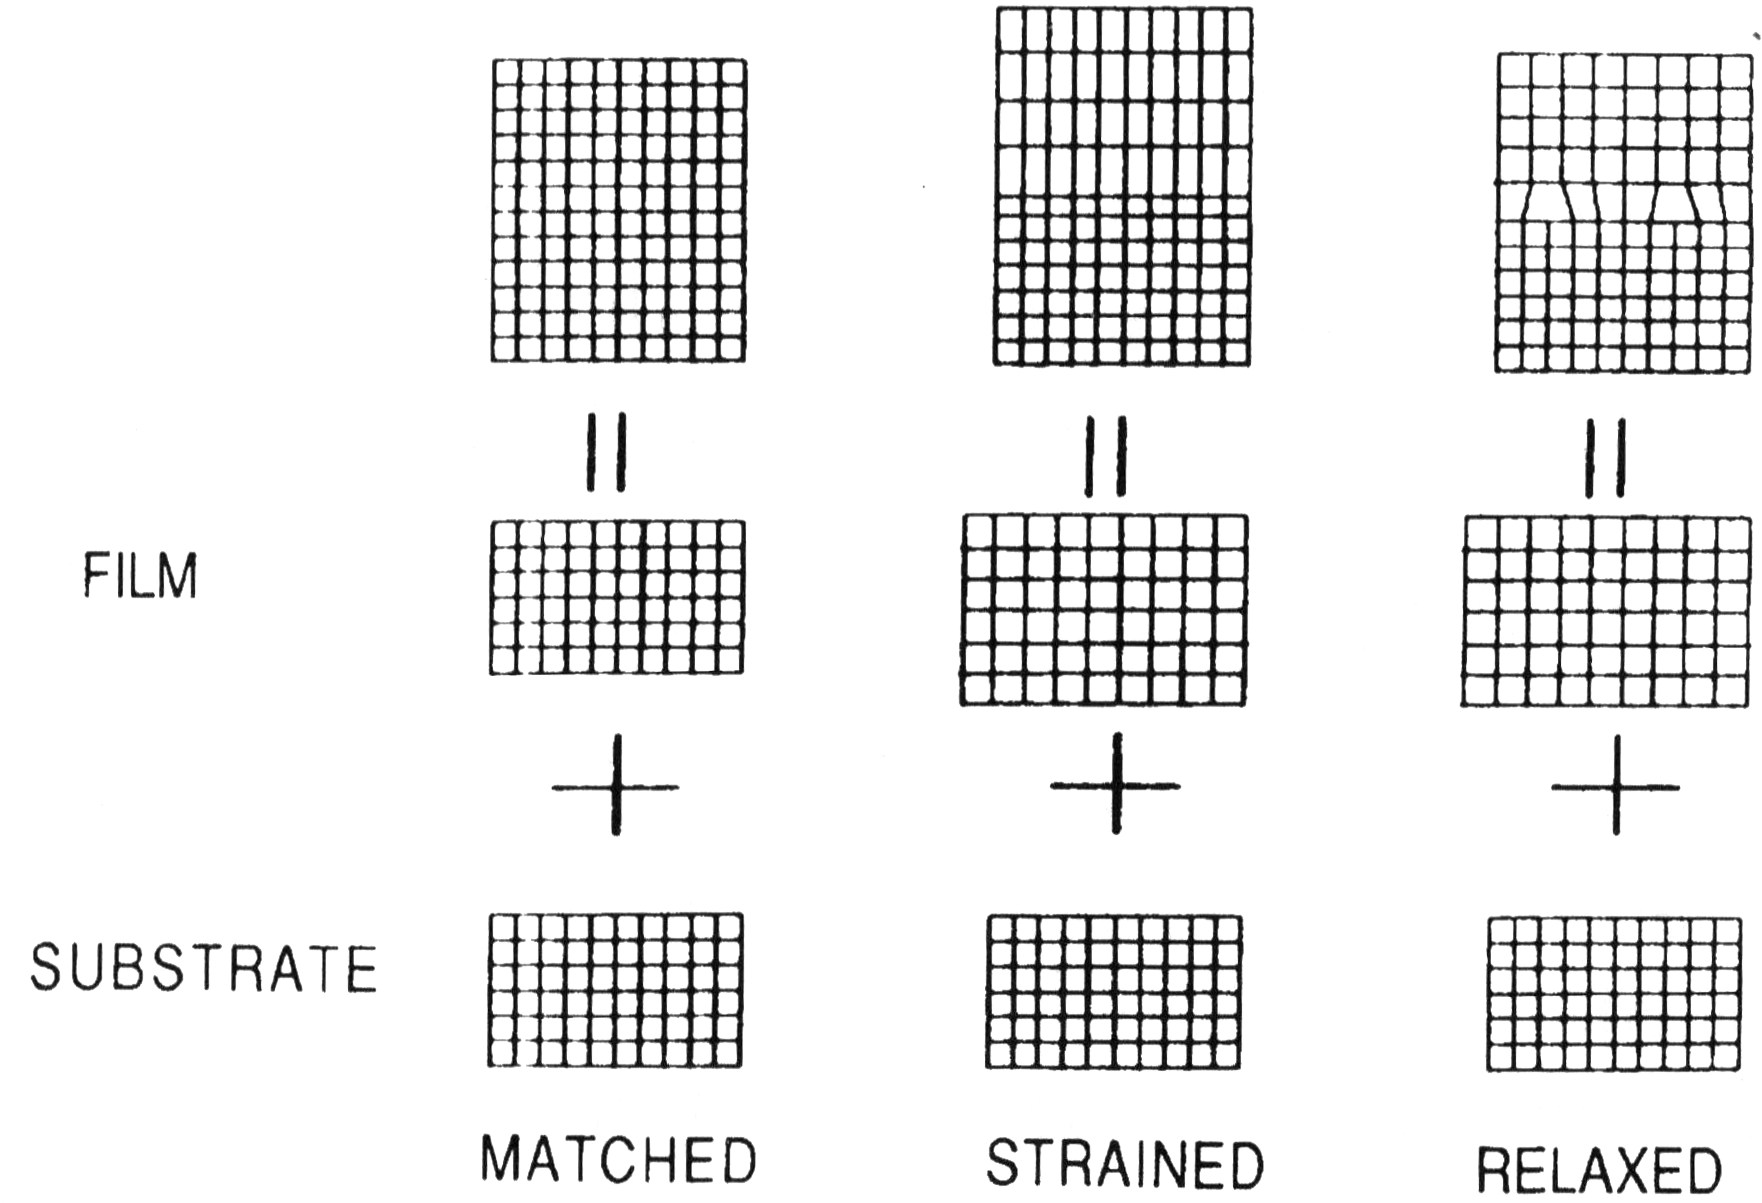
\includegraphics[width=0.7\textwidth]{back_strain}
    \caption{\label{fig:back_strain}Unit cell models of matched, strained and relaxed films from \cite{ohring2001materials}}
\end{figure}
\begin{figure}
    \centering
    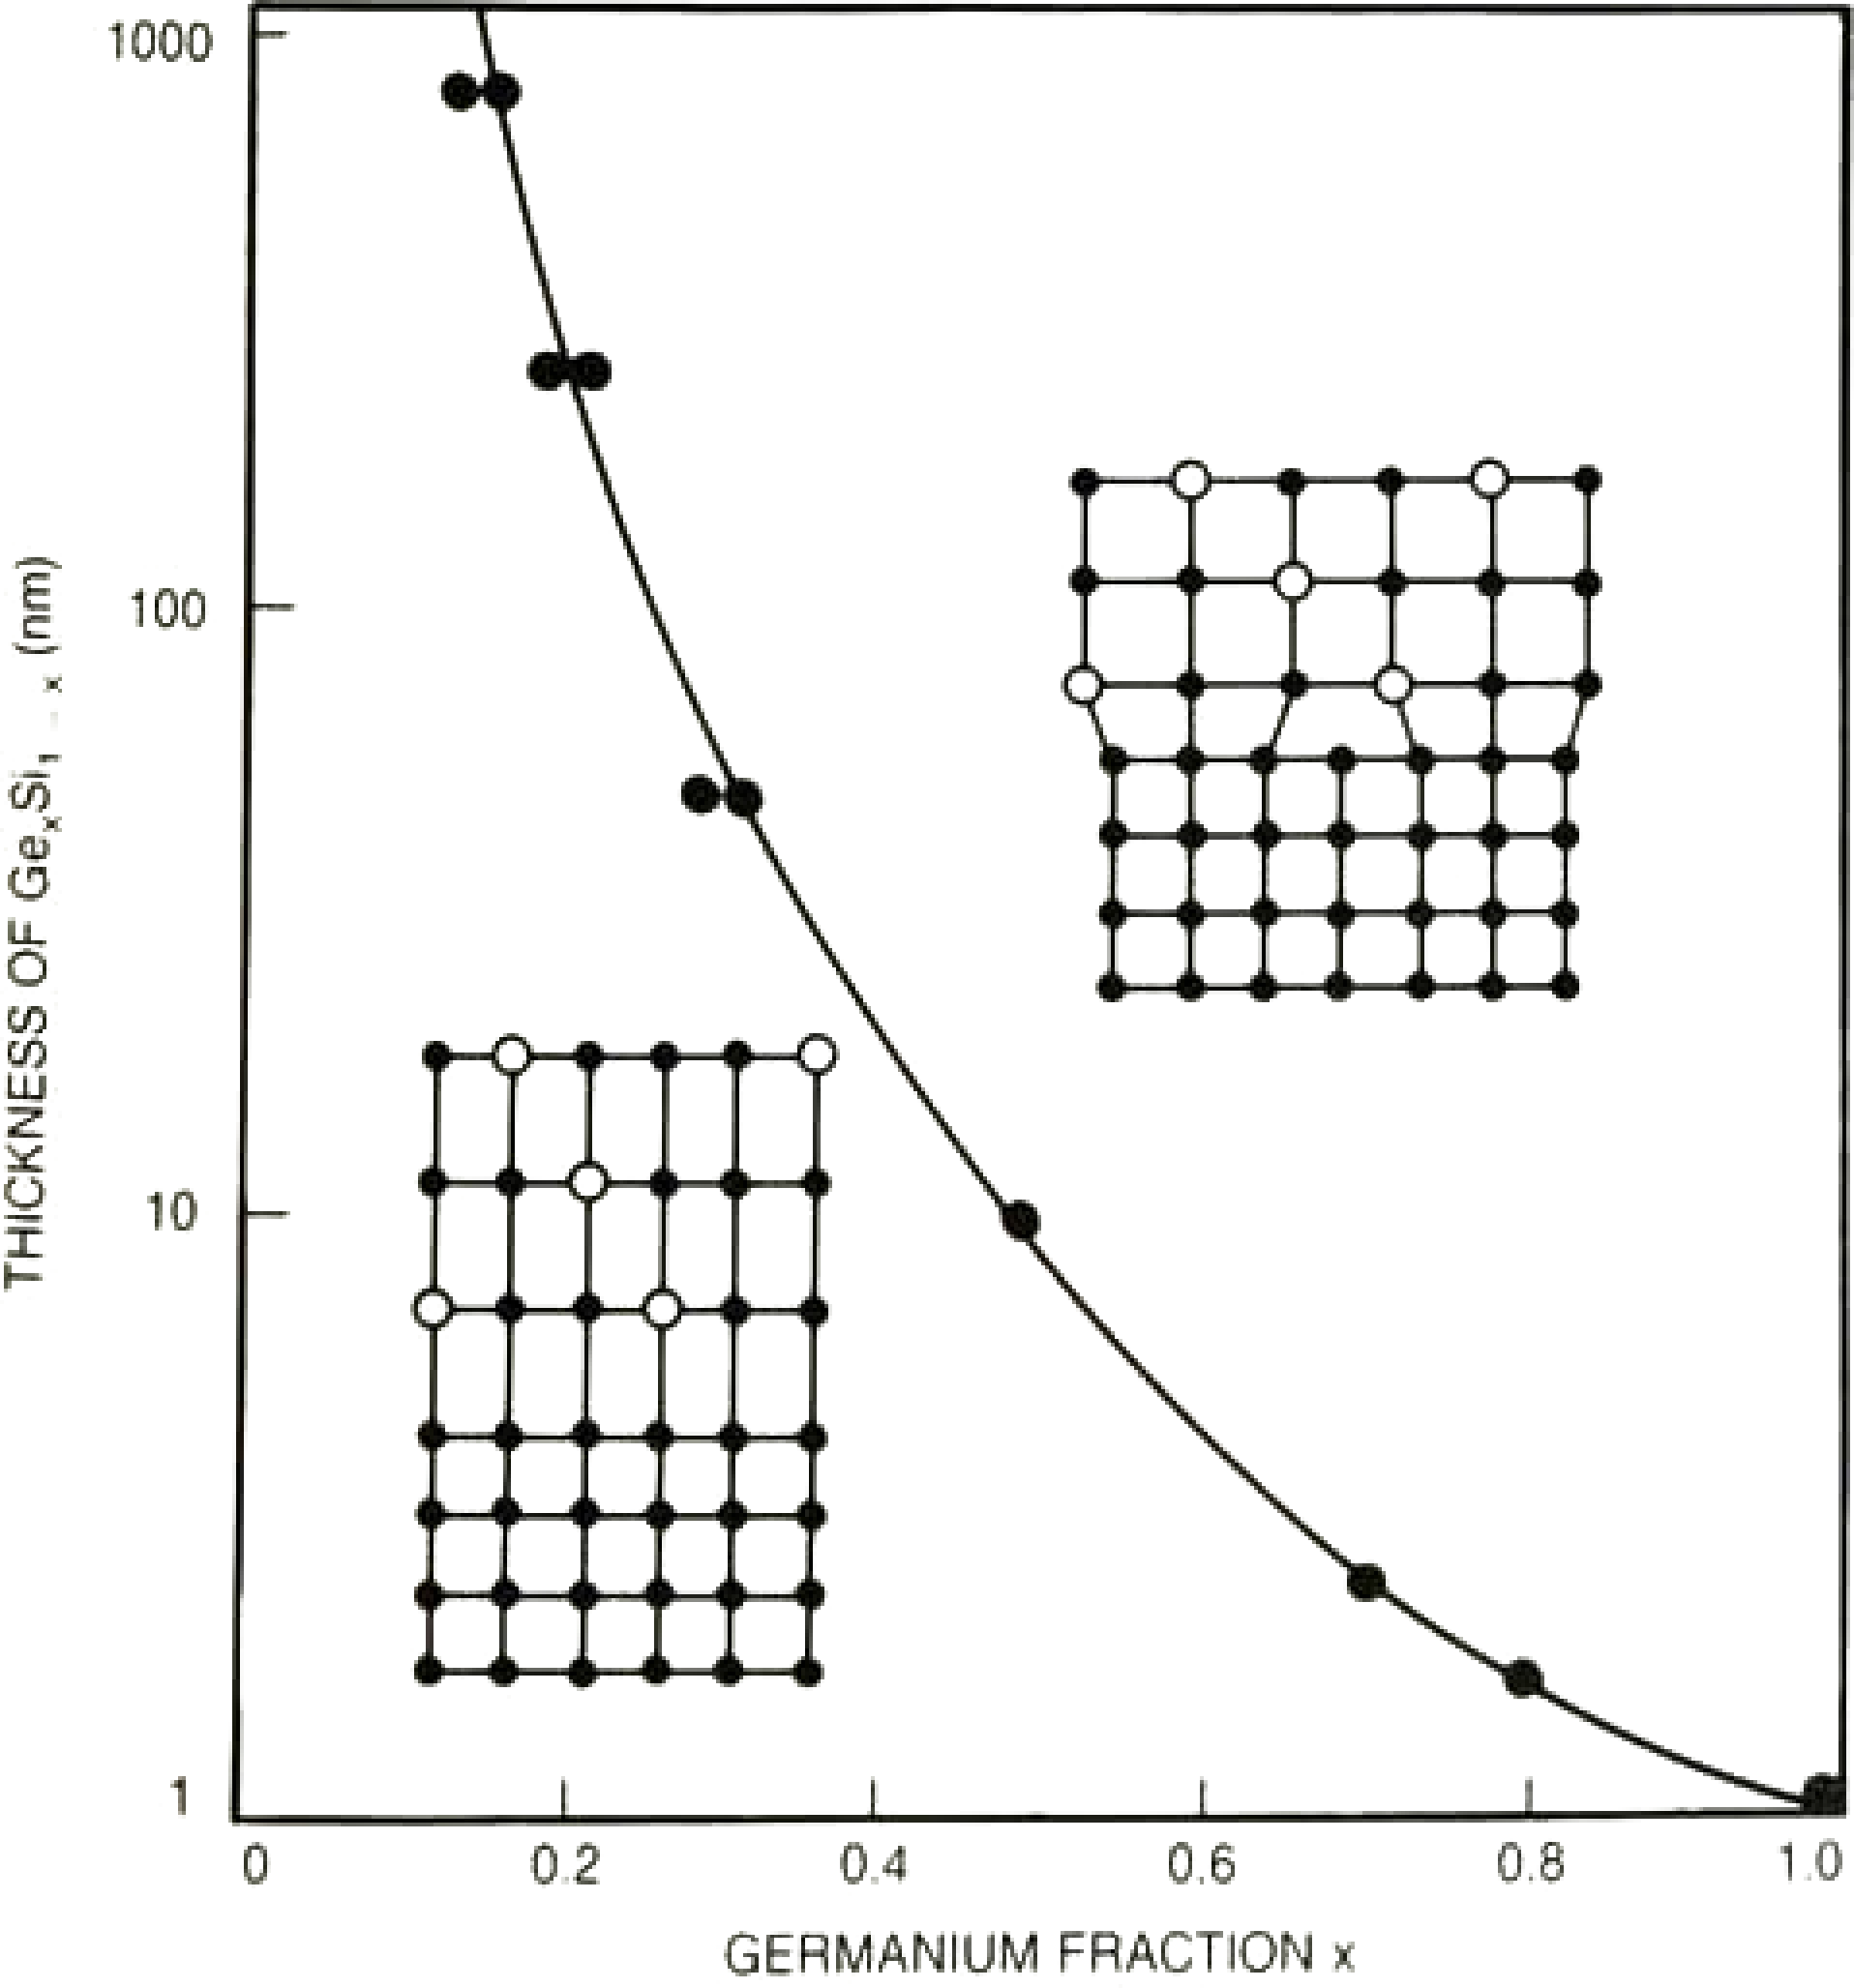
\includegraphics[width=0.9\textwidth]{back_strain_regions}
    \caption{\label{fig:back_strain_regions}Regions of pseudomorphic and relaxed growth versus lattice mismatch}
\end{figure}
\begin{equation}
f = \frac{a_f - a_s}{a_s} \label{eqn:strain}
\end{equation}
%* Matched
%* Strained
%* Relaxed films
%Pseudomorphic growth
%Relaxation via defects
%Misfit dislocation


\subsection{Clusters and Nucleation}
\begin{figure}
    \centering
    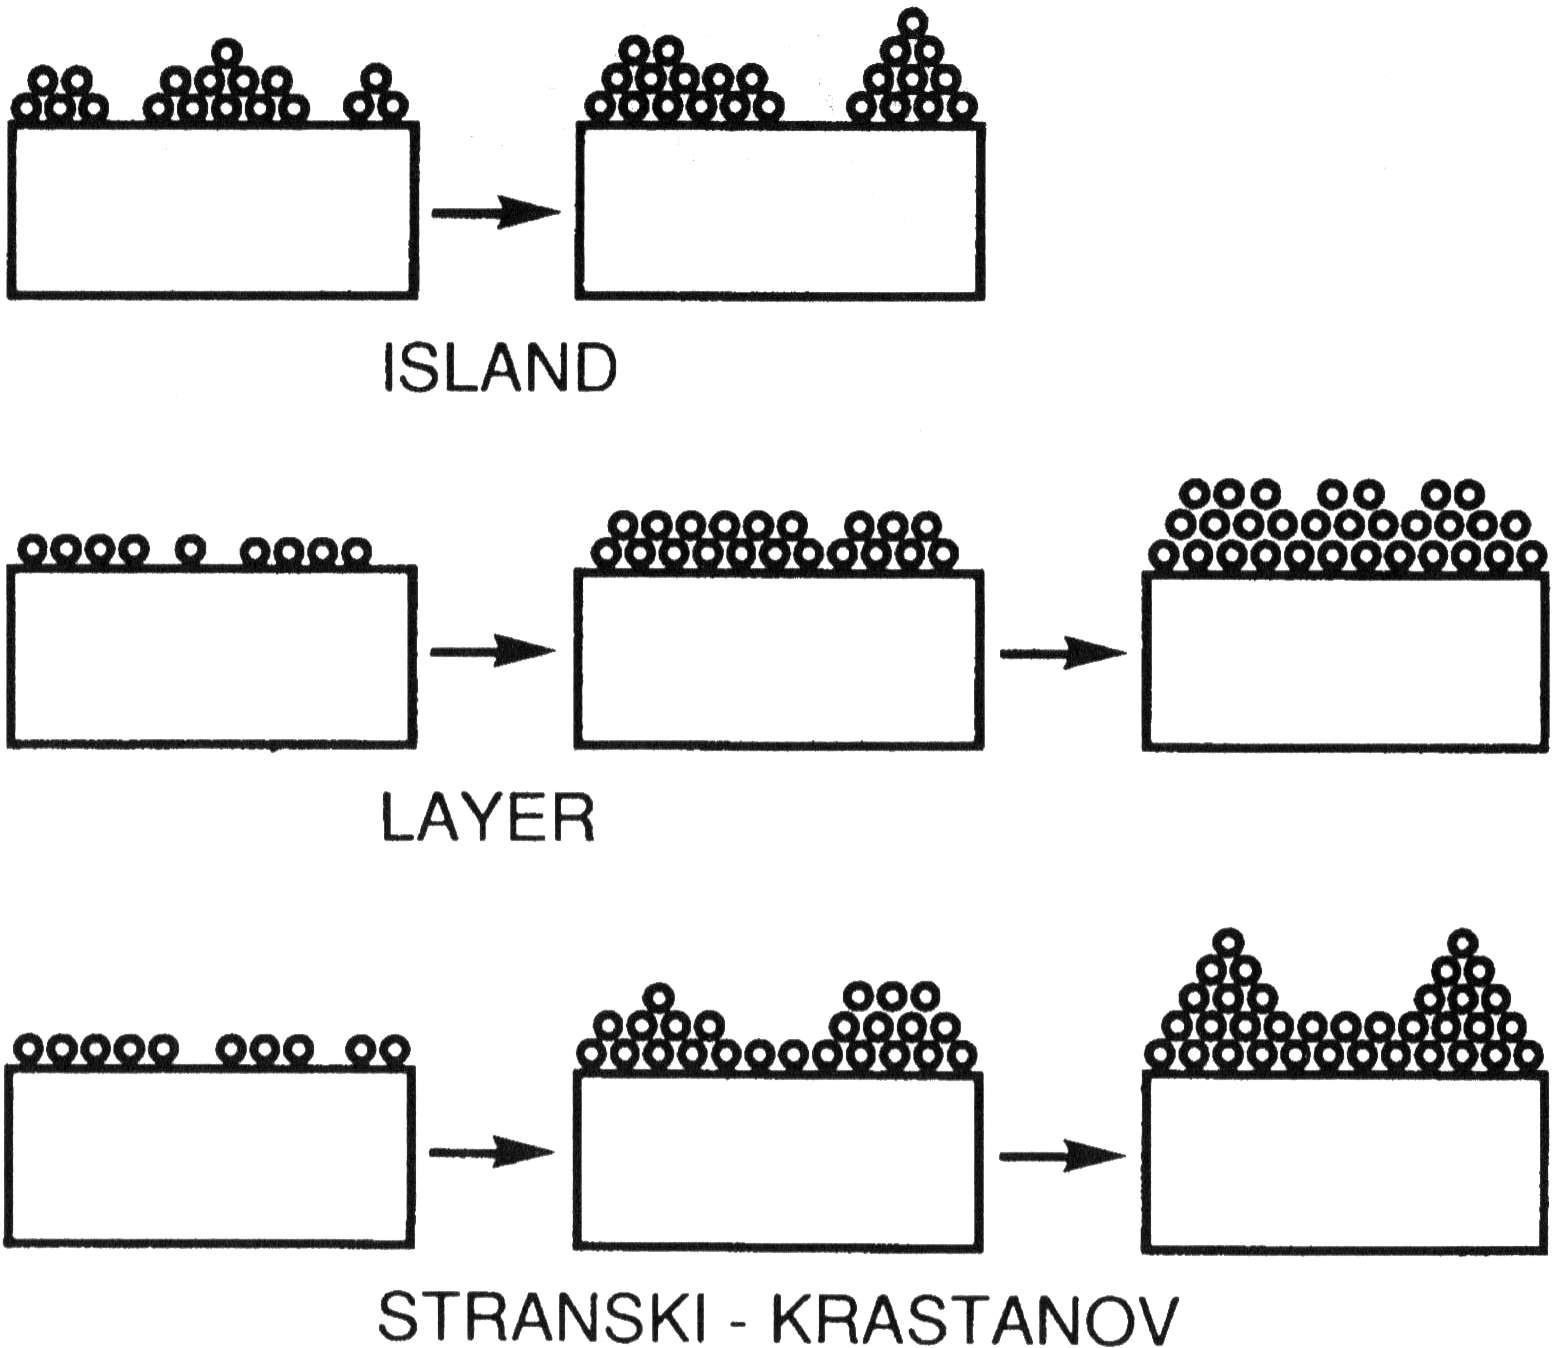
\includegraphics[width=0.7\textwidth]{back_growth_mode}
    \caption{\label{fig:back_growth_mode}SK, layer-by-layer and frank van der mere growth modes\cite{ohring2001materials}}
\end{figure}

\begin{figure}
    \centering
    \missingfigure{pg 383 regions of types of growth}
    \caption{\label{fig:back_nucleation_regions}Figure from Ohring page 383}
\end{figure}

\section{Surface Reconstructions} 
If one were to consider a crystal of infinite size, and subsequently cut it along any direction, the resulting surface would be a very high energy surface. Bonds will be completely unsatisfied (truncated electron clouds), there is likely to be an unbalanced charge, and the surrounding environment for each surface atom will be significantly different than they were in the bulk. This high energy condition is clearly not the equilibrium state and must be resolved. The resolution of this high energy state that results when surfaces of a single crystal are exposed is called the surface reconstruction. While the name surface reconstruction implies changes to just the surface atoms, the surface reconstruction can extend a number of layers into crystal. Thus, the changes that occur at the surface of a crystal can result in a very different interface than the bulk crystal for the purposes of epitaxy.

The atoms on the surface of a newly cleaved crystal have a number of options for resolving their high energy configuration. The simplest of options for atoms in those high energy states to reduce their energy is to move, that is, to change it's position relative to other atoms. These movements happen both the in-plane and out-of-plane directions. Both atomic translations can cause additional shifts in the atomic layers below the surface.  Both in-plane and out-of-plane atomic movement breaks the bulk symmetry of the original crystal, resulting in a surface with lower symmetry. In extreme cases, atoms can migrate and form islands or otherwise cause faceting on the surface in order to minimize energy. A schematic example of the atom movement for surface reconstruction is shown in \cref{fig:back_recon_move}.
\begin{figure}
    \centering
    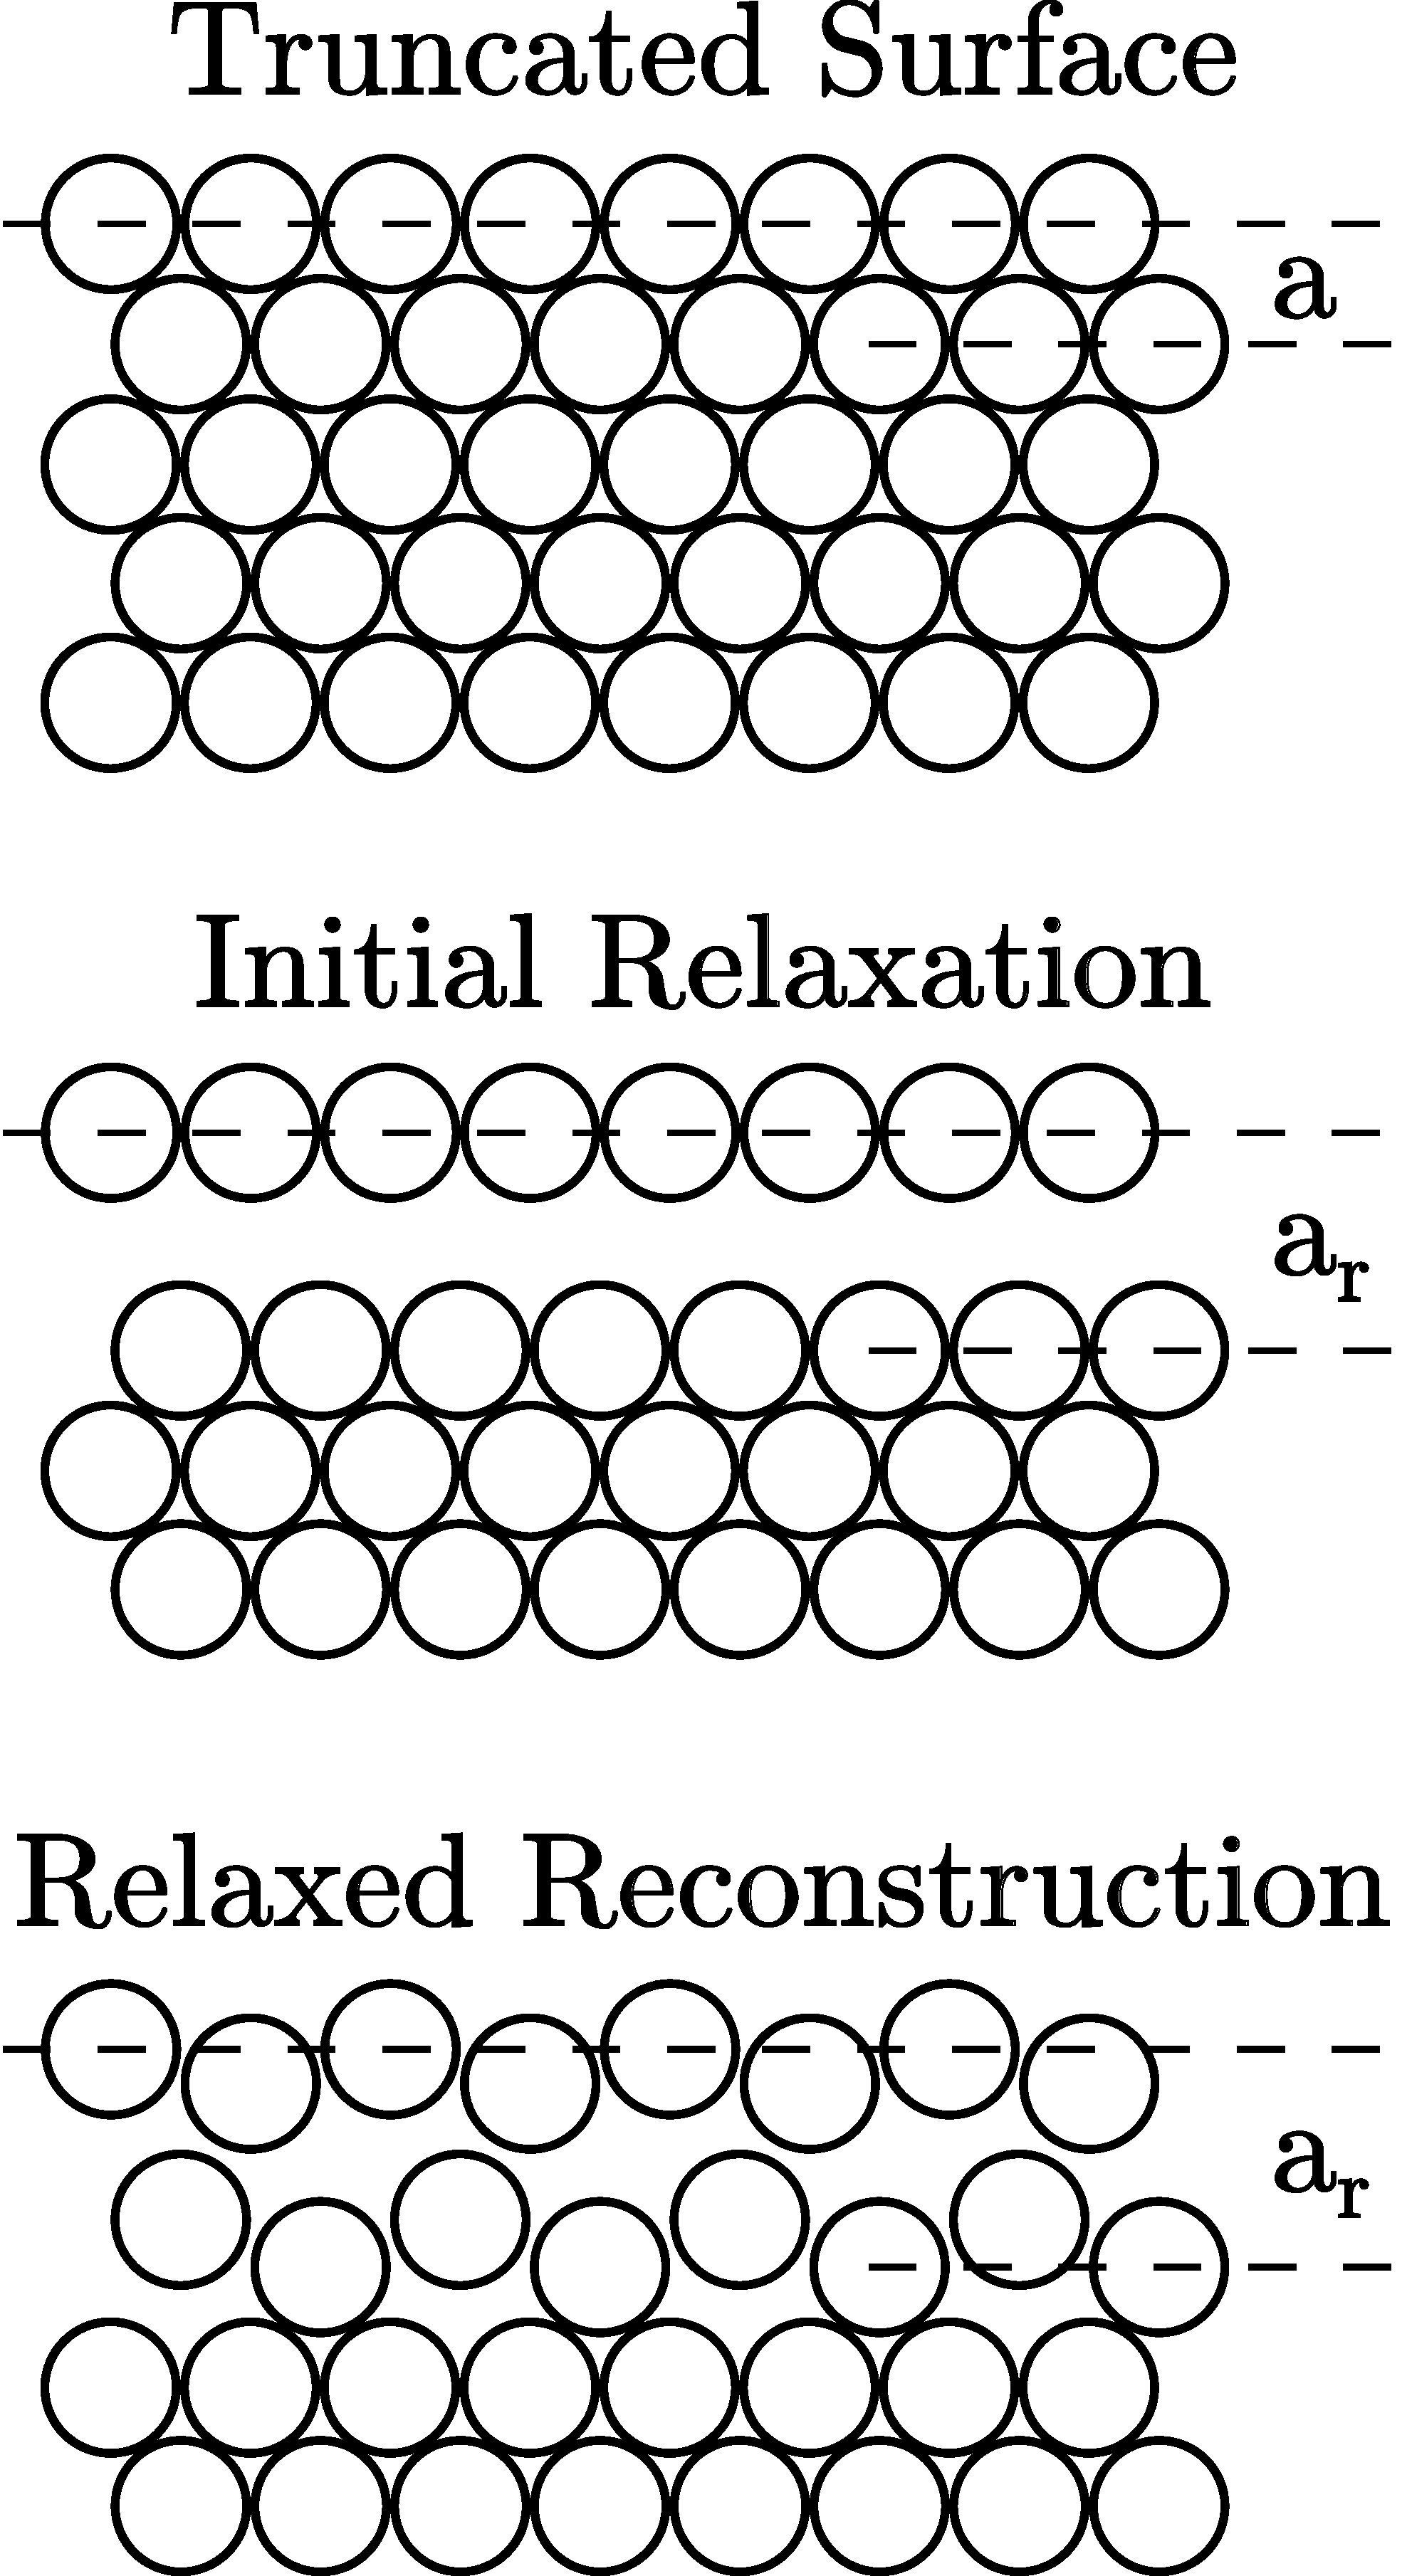
\includegraphics[width=0.7\textwidth]{back_recon_move}
    \caption{\label{fig:back_recon_move}Example of surface reconstruction with atomic movement}
\end{figure}

A more complex response resulting in a surface reconstruction that can arise is a change in the actual bonding in the upper layers of the crystal. Dimers and higher order bonding can form at the surface of the crystal, partially resolving the dangling bonds present on the surface. This dimerization of the surface can significantly reduce the chemical activity of the surface since the electronic structure has been satisfied internally to the crystal. An example of such dimerization is shown in \cref{fig:back_recon_dimer}
\begin{figure}
    \centering
    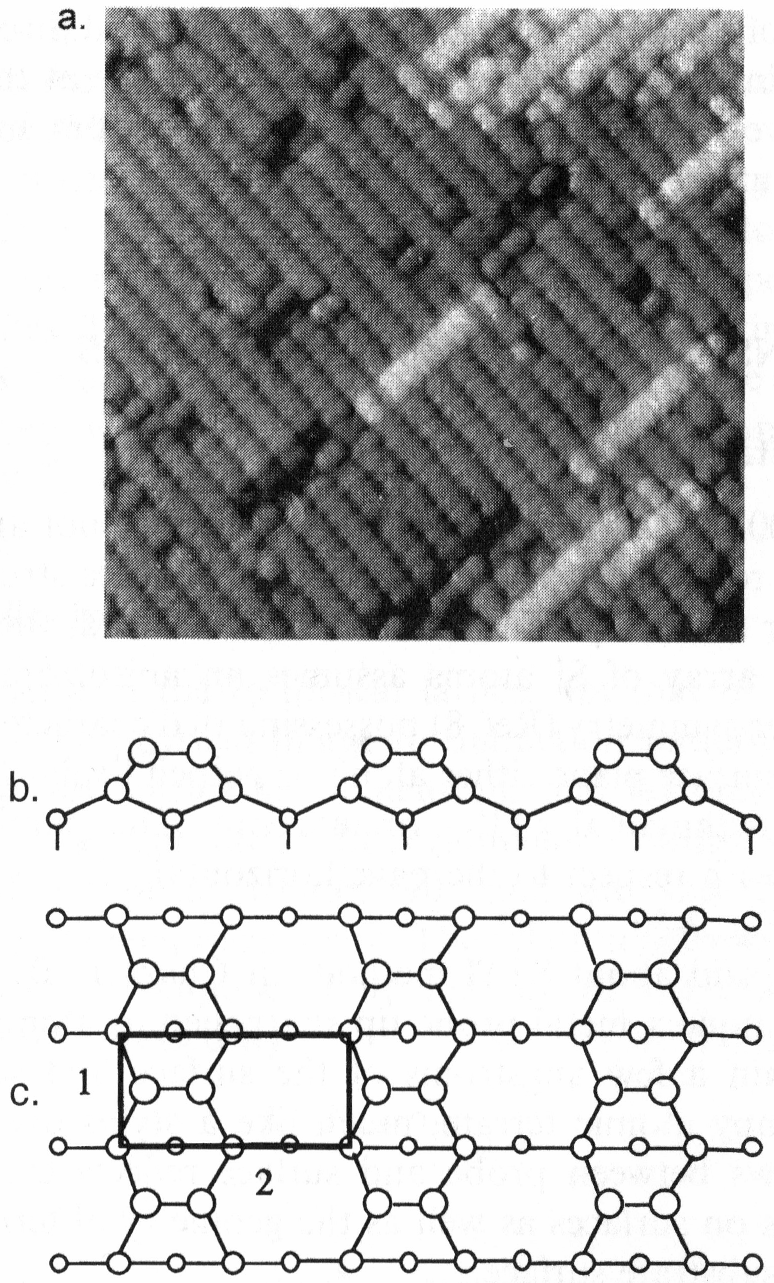
\includegraphics[width=0.7\textwidth]{back_recon_dimer}
    \caption{\label{fig:back_recon_dimer}a) STM of silicon surface reconstruction showing dimers b) cross sectional view of model ($2 \times 1$) surface reconstruction c) top view showing reconstructed surface unit cell \cite{ohring35}} 
\end{figure}

Finally, a surface can reconstruct by losing some of the atoms which originally formed the surface. The removal of such atoms can allow which was once a close-packed surface to have significantly less density than the parent crystal lattice.

\subsection{Cuts along high-index planes}
When crystals are cut along low index planes (100,111,110), surface reconstructions happen directly on these surfaces. When crystals are cut along high index planes, there is additional energy associated with exposing non-close-packed planes. These high index planes are highly unfavourable and do not have stable reconstructions. The high index surface instead undergoes a breakup into sections of low index planes, separated by steps of fractional or multiples of the unit cell, as shown in \cref{fig:back_recon_vicinal}. These low index planes can then further reconstruct as previously discussed.
\begin{figure}
    \centering
    \missingfigure{Vicinal surface showing reconstruction}
    \caption{\label{fig:back_recon_vicinal}Vicinal surface showing reconstruction}
\end{figure}

The most common case of high index planes exposed for surface reconstruction is offcut or vicinal surfaces. The surfaces of single crystal wafers, when cut from a boule have a misalignment from the intended low-index plane due to processing error. These wafers, when reconstructed form terraces of the low index plane, separated by fractional unit cell steps.

\subsection{Thermodynamics, Kinetics and Stability of Surface Reconstructions}
While a unreconstructed crystal surface is in a high energy state, all the routes to lower energy states require an input of energy. Thus, while a crystal surface may be in a relatively high energy state after cutting, cleaving, polishing or other processing which exposes that surface, it can do very little to resolve its situation without help. Energy must be inputted into the system in order to allow the atoms to move, bond or leave the surface. The energy landscape of surface reconstructions has many local minima, so there are many possible surface reconstructions for a given surface, depending upon how much activation energy is provided to the system. Beyond how much energy is delivered to the crystal, it takes time for the atoms to reach a one of local minima for the surface. Some surface reconstructions can take a significant time to achieve, adding more energy would result in transitions into another reconstruction so the only route is time.

Thus far, energy and time have only been discussed in general terms. The most successful and commonly used method of actually delivering energy and eliciting a reconstruction is to increase the temperature of the crystal. Annealing crystals can be done at a carefully controlled temperature for any desired amount of time. Careful experimentation with various crystals has resulted in ``phase diagrams'' of surface reconstructions given a surface and temperature combination, as seen in \cref{fig:back_recon_phase}.
\begin{figure}
    \centering
    \missingfigure{Phase diagram of surface reconstruction}
    \caption{\label{fig:back_recon_phase}Phase diagram of surface reconstruction}
\end{figure}

The formation and stability of a given surface reconstruction also depends upon the environment surrounding the crystal. Assuming the surrounding environment does not chemically react with a given crystal, the presence of absence (vacuum) of an inert gas will affect the activation energies for the surface atom processes. A vacuum above a crystal when annealing promotes the exit of atoms from the surface as there is force resisting the atoms, or back scattering them towards the surface. For complex crystals which incorporate elemental gasses into their lattice, different surface reconstructions are achievable if an overpressure of those gasses are present, rather than a vacuum. These surface reconstructions are commonly seen in the complex oxides, where oxygen is a primary constituent of the crystal and will be lost from the surface during annealing if an overpressure is not provided.

Stability of surface reconstructions to subsequent interactions with atoms added to the surface varies widely depending upon the properties of the crystal. Semiconductor crystals have less stable surface reconstructions, interactions with additional atoms easily destroy an established reconstruction. Refractory crystals such as complex oxides are considerably more stable once reconstructed, a point which has been taken advantage of in this work.

\subsection{Nomenclature for Surface Reconstructions}
Since surface reconstructions are pseudo-2D constructs, the allowed symmetries of a surface reconstruction are a subset of those of the allowable 3D lattices. There are five unique 2D surface nets that can be used to describe the symmetry of a surface reconstruction as shown in \cref{fig:back_recon_lattices}
\begin{figure}
    \centering
    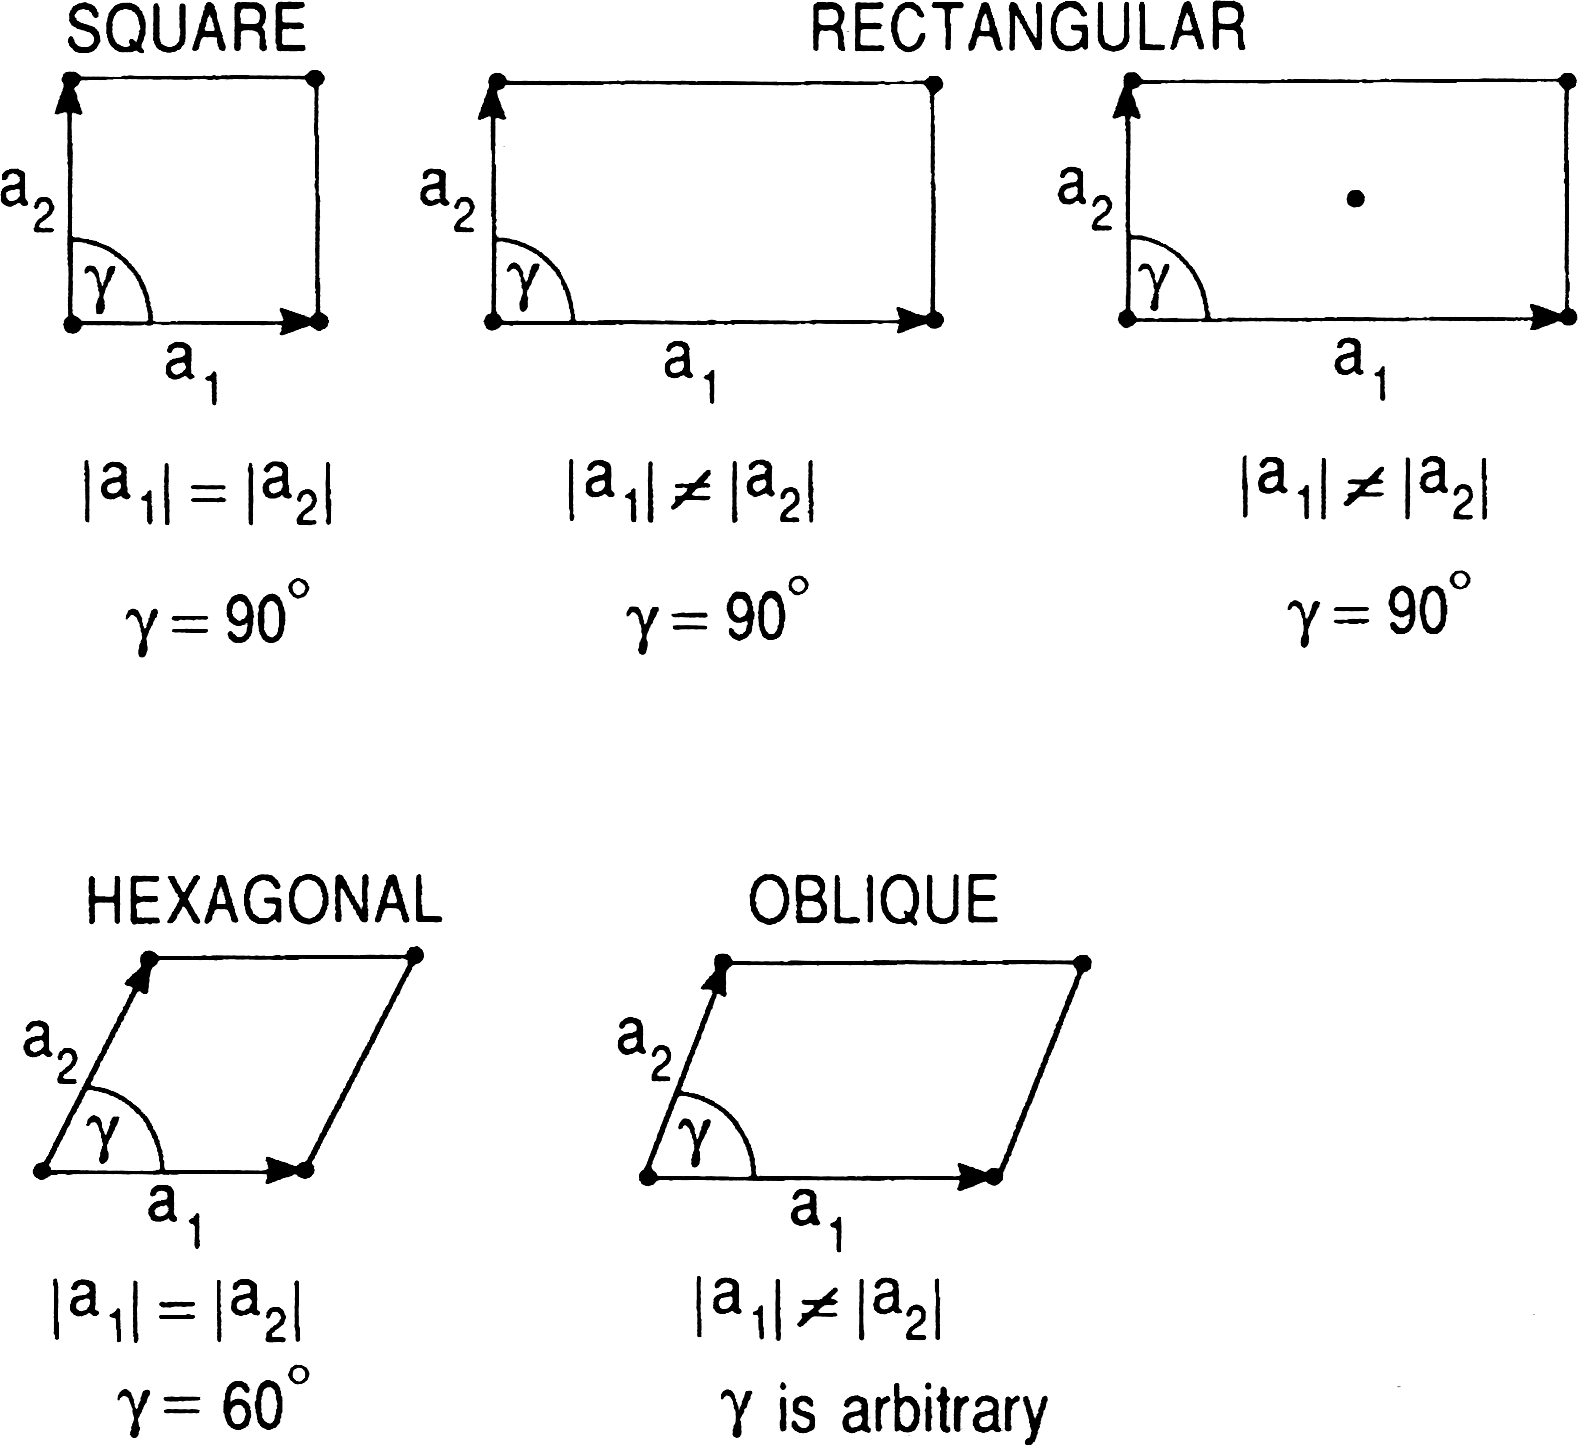
\includegraphics[width=0.8\textwidth]{back_recon_lattices}
    \caption{\label{fig:back_recon_lattices}The five unique 2D surface nets (figure7-6)}
\end{figure}

The nomenclature of naming surface reconstructions is determined by the relationship of the 2D surface lattice to the underlying unit cell. The smallest repeating surface cell is determined and denoted by whether it is primitive (P), having only one atom per surface cell, or centred (C). The surface cell's repeat unit is then related to underlying unit cell by the ratio of the surface cell lattice constant to the unit cell lattice constant. Thus, the simplest surface reconstruction for a crystal would be the P($1 \times 1$) reconstruction, containing one atom, and having the same spacing as then underlying crystal. These nomenclatures do not include details such as the type, number or configuration of atoms which make up the reconstruction. These reconstructions can also be rotated relative to the underlying unit cell being denoted by R. A number of example surface reconstructions namings are shown in \cref{fig:back_recon_name_examples}. The nomenclature for surface reconstructions is not unique, as a reconstruction such as C($2\times2$) is equivalent to ($\sqrt{2}\times\sqrt{2}$)R45\degree~reconstruction.
\begin{figure}
    \centering\
    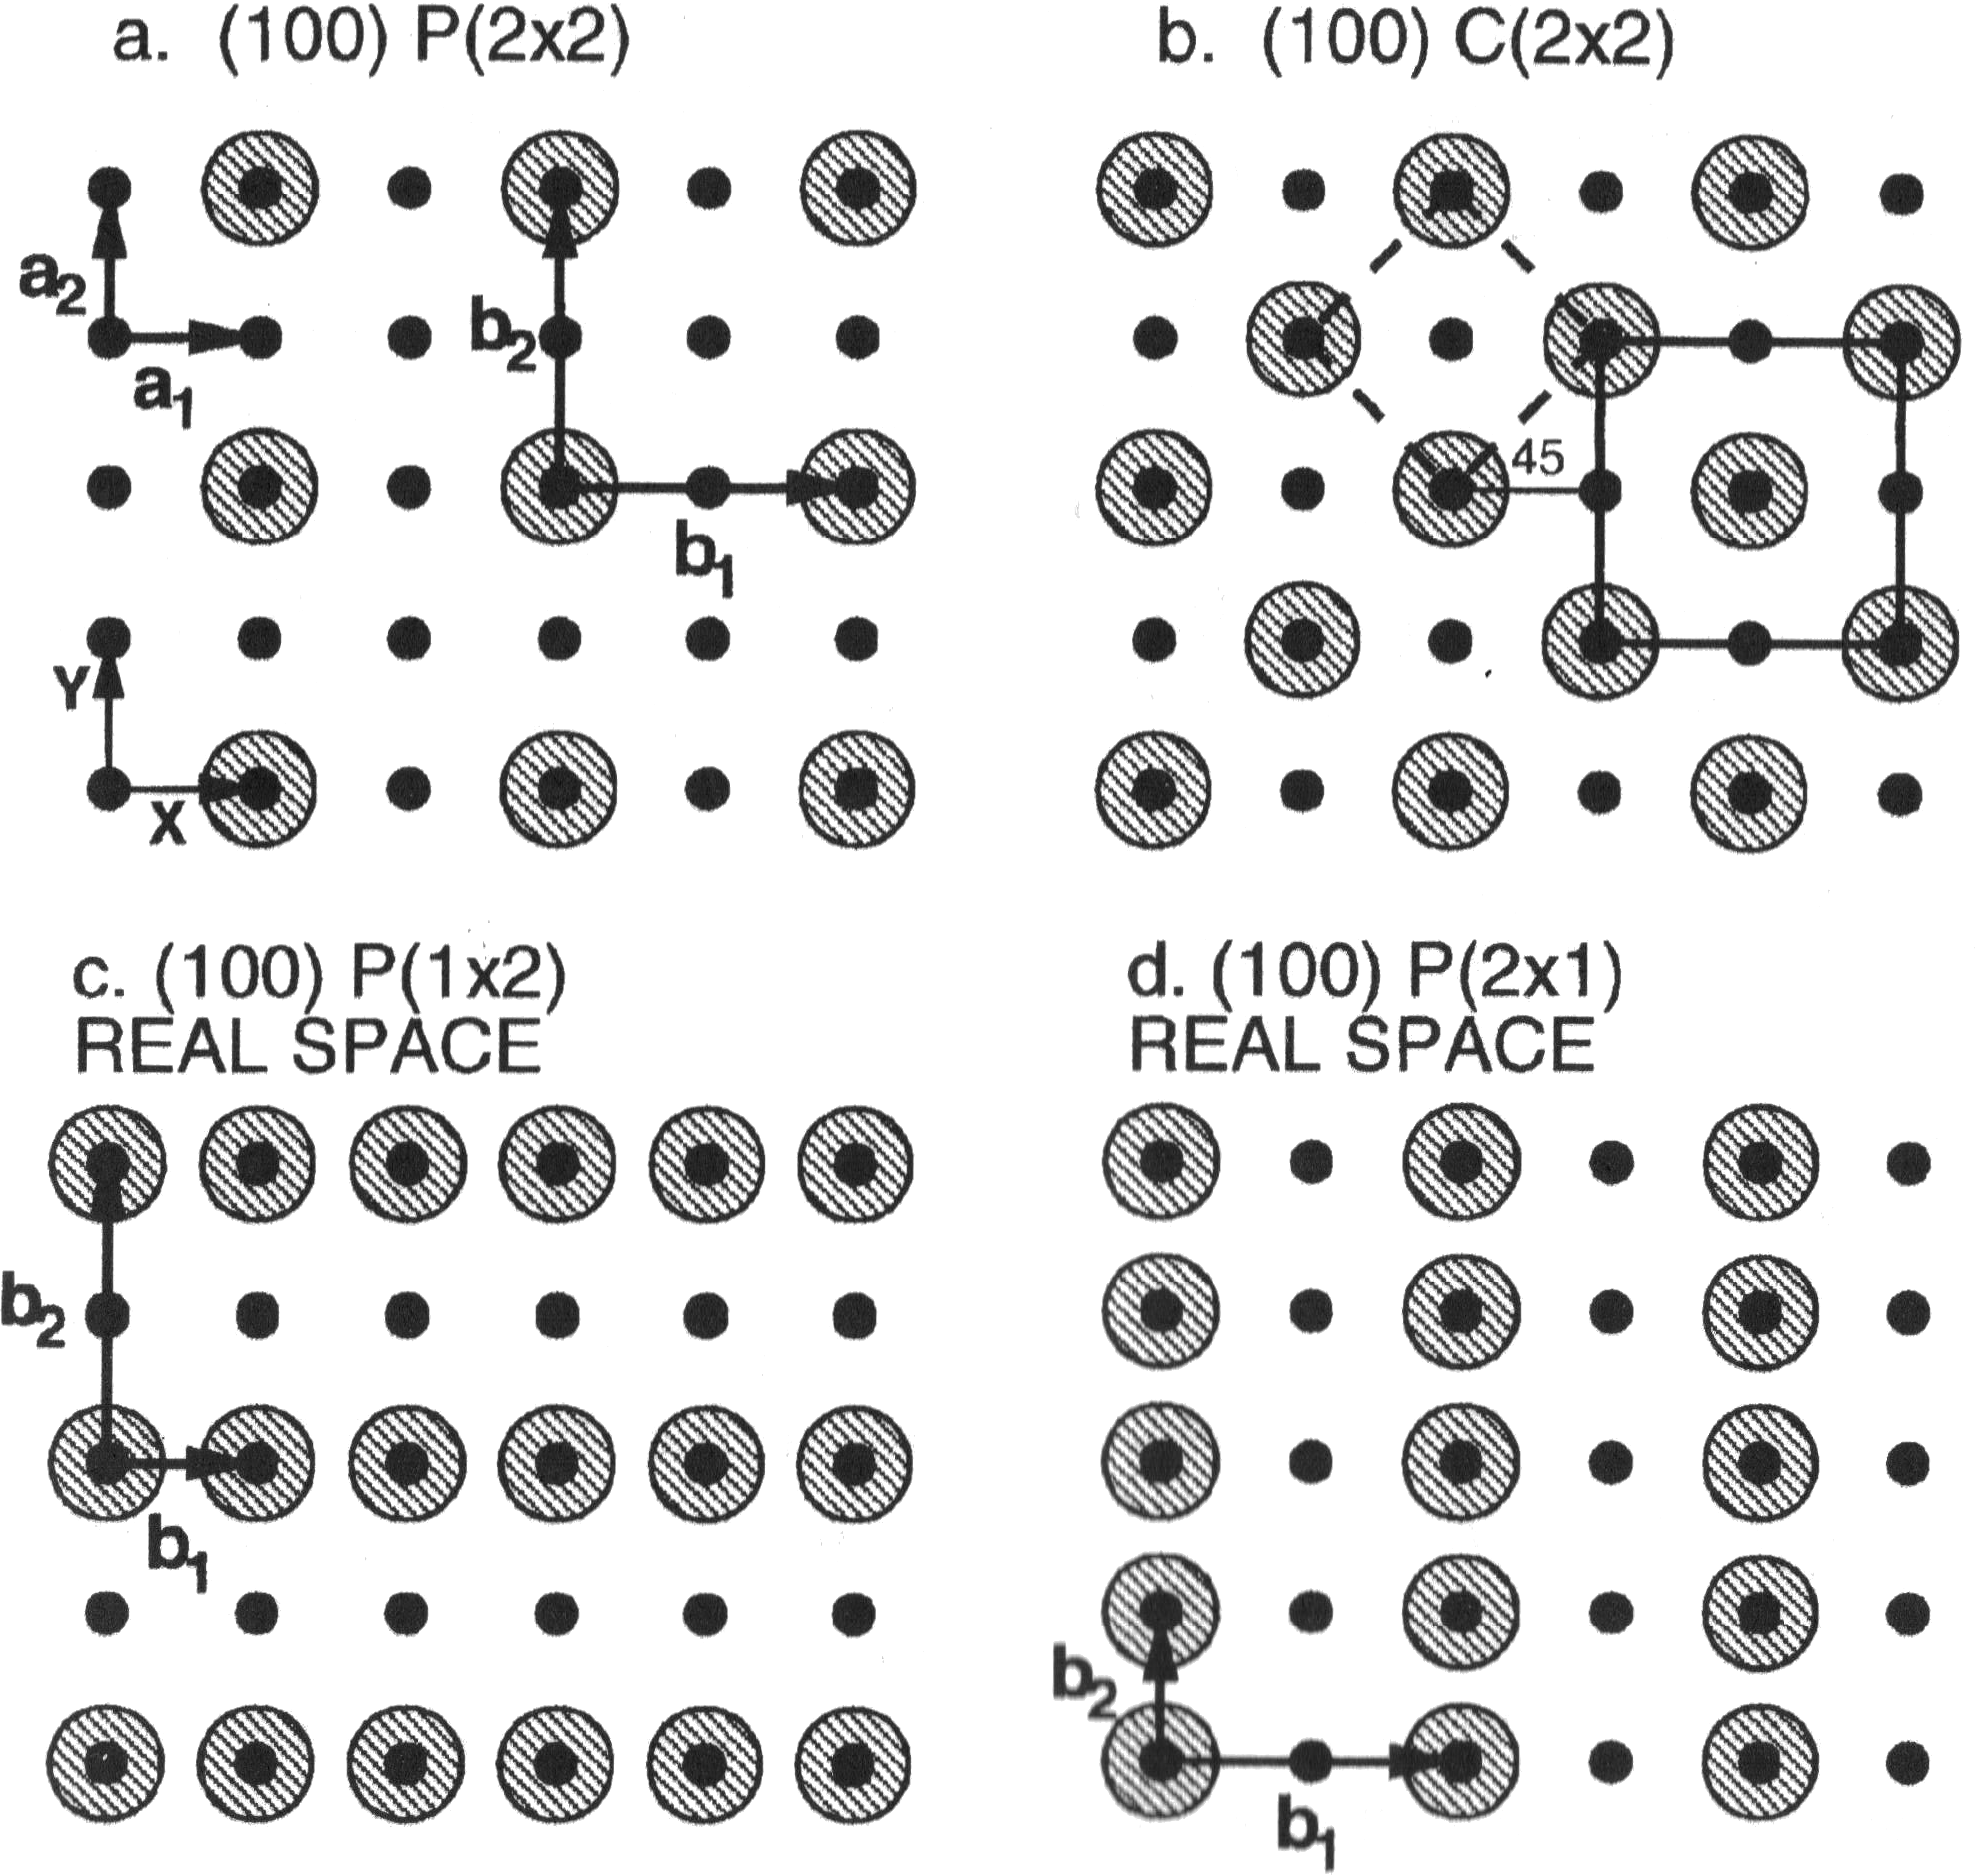
\includegraphics[width=0.9\textwidth]{back_recon_name_examples}
    \caption{\label{fig:back_recon_name_examples} Atomic positions of adatoms (shaded) relative to atoms (dots) arrayed on a (100) simple cubic substrate. a) P($2 \times 2$) b) C($2 \times 2$) or ($\sqrt{2}\times\sqrt{2}$)R45\degree c) P($1 \times 2$) d) P($2 \times 1$)}
\end{figure}

\section{Atomic Bonding}
\begin{figure}
    \centering
    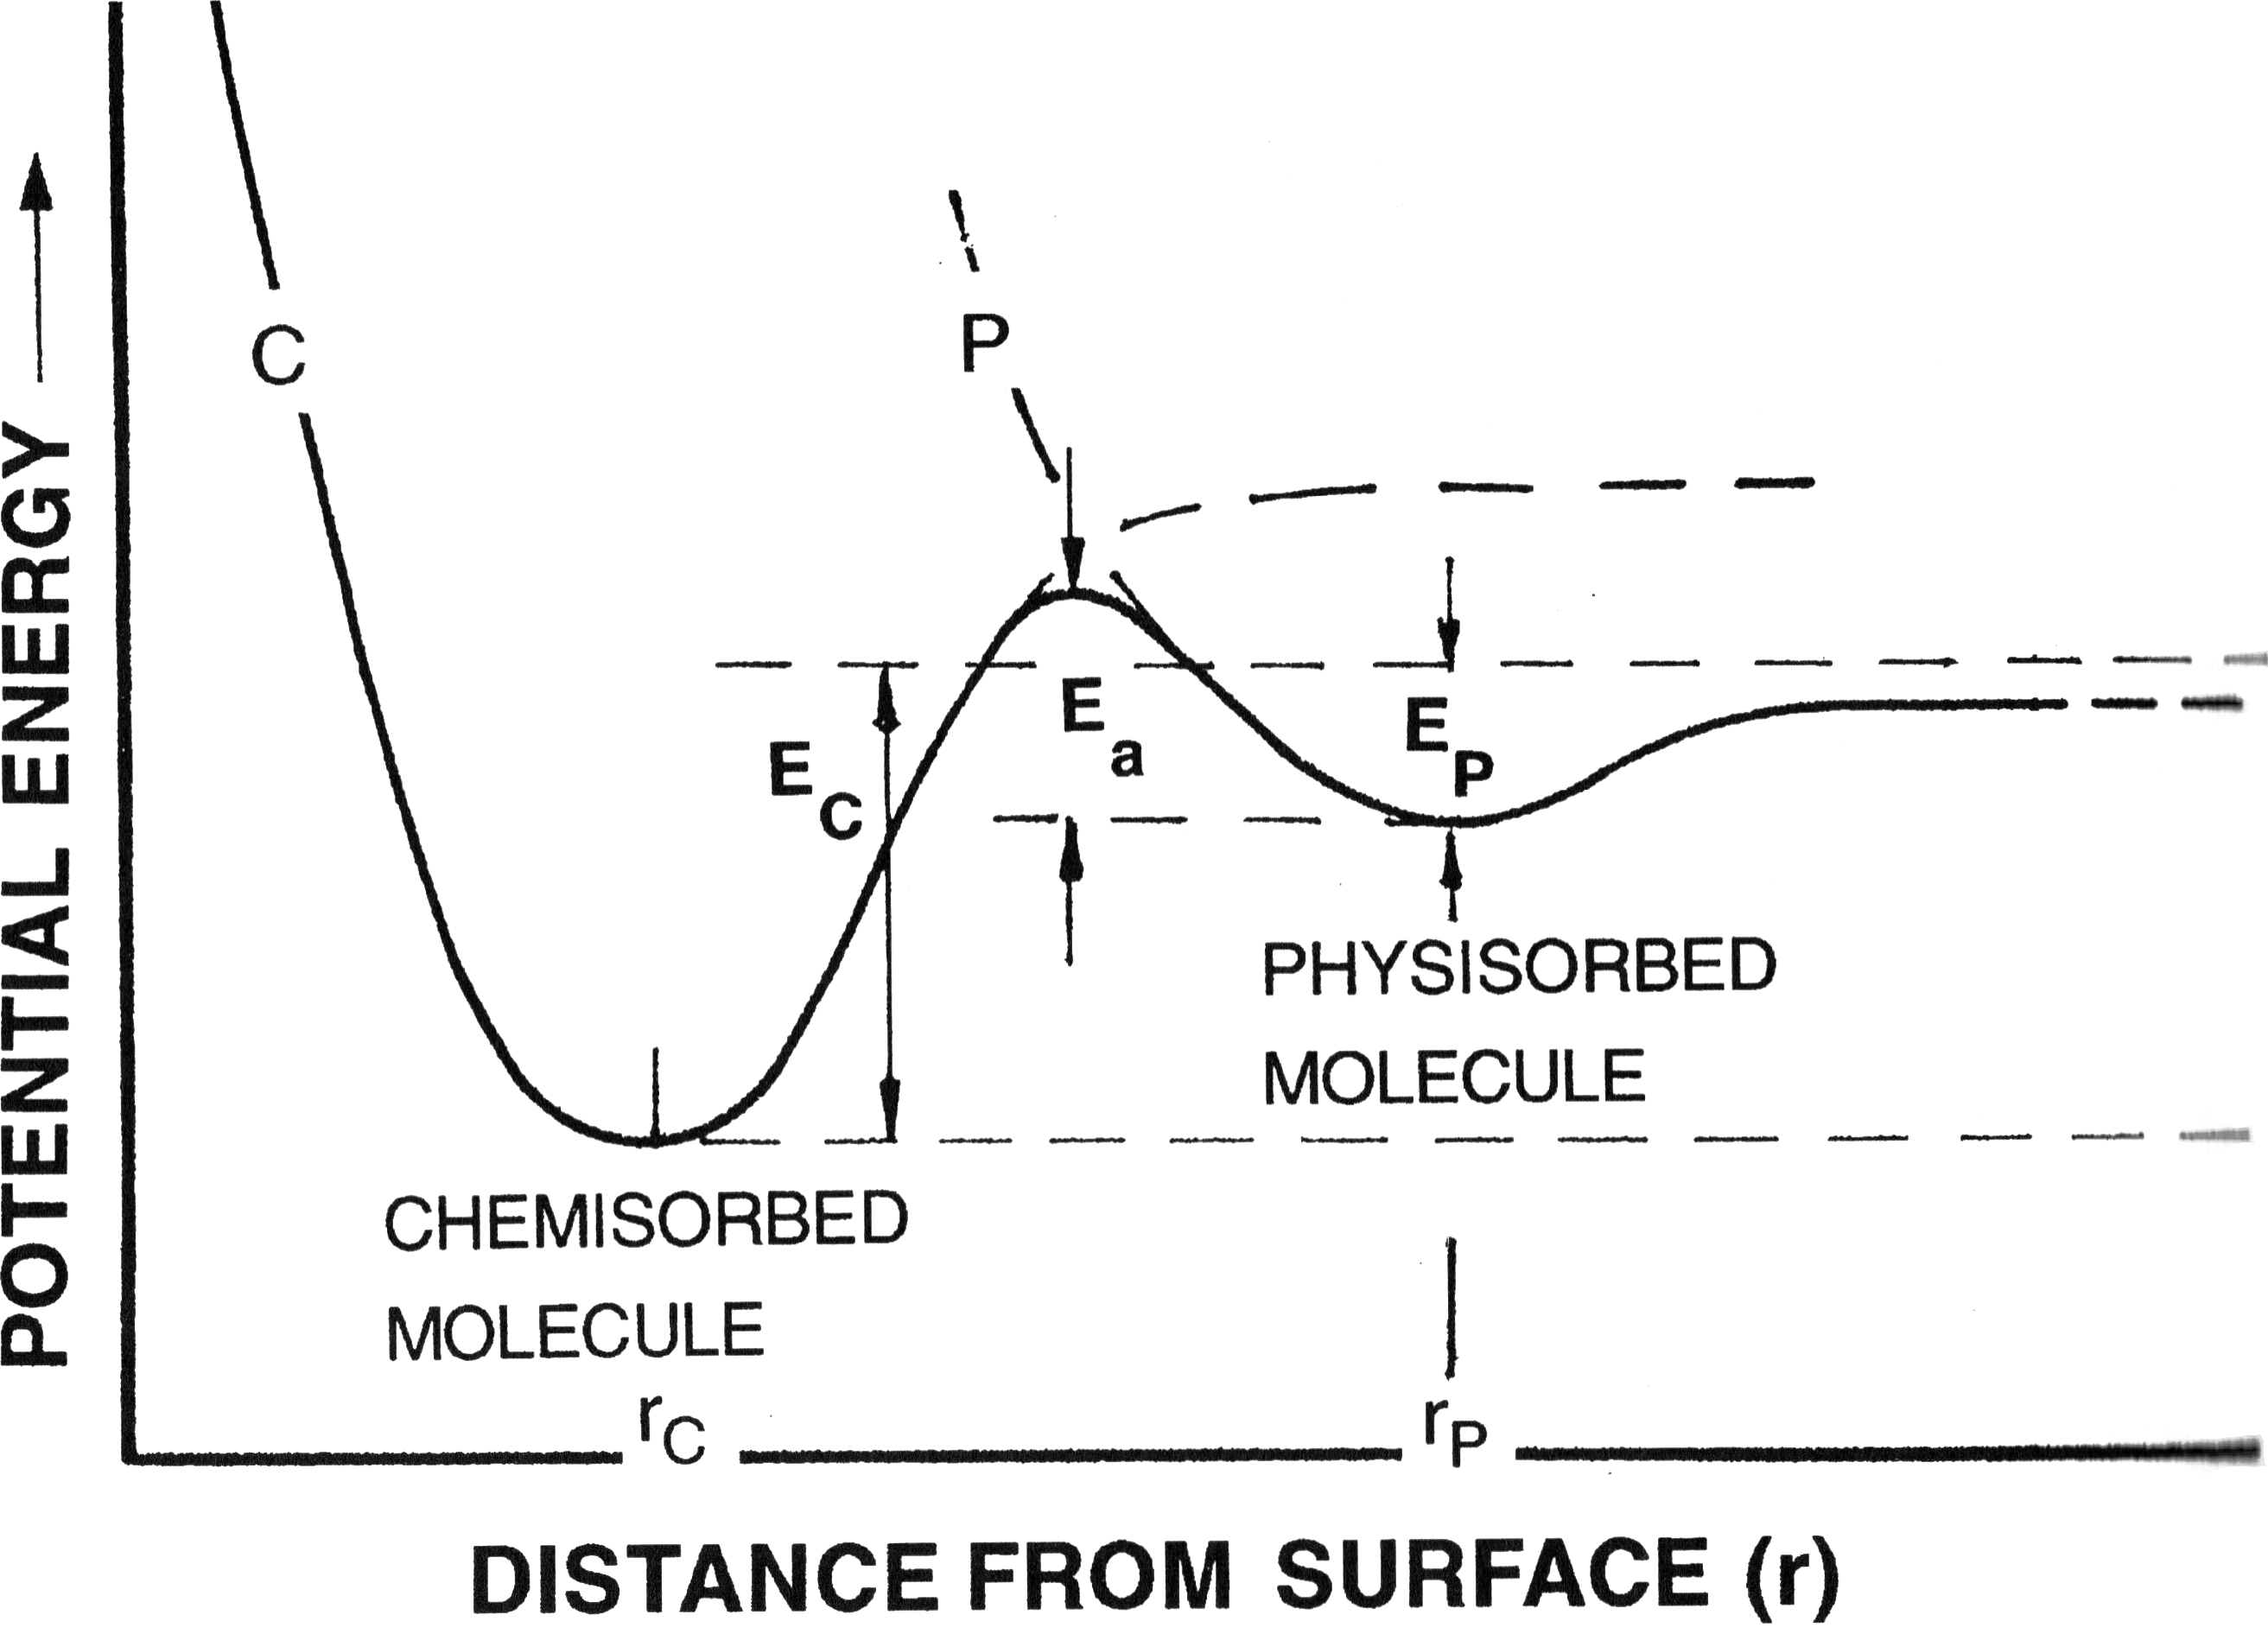
\includegraphics[width=0.9\textwidth]{back_bond_potential}
    \caption{\label{fig:back_bond_potential}Potential energy versus distance for atom respect to surface}
\end{figure}

